% =====================================================================
%  RAPPORT — Groupe 5, Projet 5 (VERSION CORRIGÉE, présentation conservée)
%  Processus gaussiens pour l'optimisation bayésienne
%  MAA4371 — Master (M1) DSIM, Université de Dschang
%
%  Cette version REPREND la présentation du rapport soumis (mise en page aérée,
%  pages de séparation, structure Objectif / Hypothèses / Lemmes / Conclusion par
%  démonstration, une formule par ligne) et y INTÈGRE les corrections :
%    * Diebold–Mariano (DM = -20) supprimé ; conclusion statistique corrigée
%    * Lemme 1 du regret : argument d'union bound ajouté
%    * Dérivation de gamma_N esquissée (au lieu d'une simple citation)
%    * Vérification du gradient + figure de stabilité numérique
%    * Cohérence min/max (UCB en max, LCB en min)
%    * Dérivation de l'Expected Improvement ajoutée
%    * Tableau de contribution ajouté
%    * Notation corrigée : X (et non E), domaine \mathcal{X} (et non Y),
%      regret r_t (et non tau_t), prior p(f) \propto ..., noyau SE avec sigma_f^2
%
%  FIGURES requises dans le même dossier :
%    numerical_stability.png  (fournie, résultat réel)
%    convergence_comparison.png , posterior_slice.png  (À REMPLACER par les vôtres)
%  BABEL : décommentez \usepackage[french]{babel} si le paquet est installé.
% =====================================================================
\documentclass[12pt]{article}

\usepackage[utf8]{inputenc}
\usepackage[T1]{fontenc}
% \usepackage[french]{babel}
\usepackage{amsmath,amssymb,amsthm,mathtools}
\usepackage{bm}
\usepackage{graphicx}
\usepackage{booktabs}
\usepackage{algorithm}
\usepackage{algpseudocode}
\usepackage[margin=1in]{geometry}
\usepackage{setspace}
\usepackage[hidelinks]{hyperref}
\onehalfspacing

\newcommand{\R}{\mathbb{R}}
\newcommand{\E}{\mathbb{E}}
\newcommand{\N}{\mathcal{N}}
\newcommand{\X}{\mathcal{X}}
\newcommand{\Hk}{\mathcal{H}_k}
\newcommand{\D}{\mathcal{D}}
\newcommand{\GP}{\mathcal{GP}}
\newcommand{\K}{K}
\newcommand{\bal}{\alpha}
\newcommand{\bth}{\theta}
\newcommand{\xs}{x^{*}}
\DeclareMathOperator*{\argmin}{arg\,min}
\DeclareMathOperator*{\argmax}{arg\,max}
\DeclareMathOperator{\tr}{Tr}
\DeclareMathOperator{\Cov}{Cov}

\newcommand{\dividerpage}[2]{%
  \newpage \thispagestyle{empty}
  \vspace*{0.32\textheight}
  \begin{center}
    {\Huge\bfseries #1}\\[14pt]
    {\Large #2}
  \end{center}
  \newpage}

\begin{document}

% =====================================================================
%  PAGE DE TITRE  (identique à la vôtre)
% =====================================================================
\begin{titlepage}
\centering
\vspace*{1.5cm}
{\Large\bfseries Université de Dschang}\\[1.2cm]
{\large Master (M1) en Data Science et Ingénierie Mathématique}\\[1.5cm]
{\large\bfseries MATHÉMATIQUE POUR L'APPRENTISSAGE AUTOMATIQUE}\\[0.8cm]
{\large\bfseries Projet}\\[0.6cm]
{\large PROCESSUS GAUSSIENS POUR L'OPTIMISATION BAYÉSIENNE}\\[1.5cm]
{\large\bfseries Participants :}\\[0.5cm]
{\large
MAHAMOUD ABDILLAHI OMAR\\[4pt]
MOHAMED ALI ABDOULKADER\\[4pt]
KOUAME YAO FRANCK\\[4pt]
MOUDINE ARMEL BOURI\\[4pt]
LAGRE GABBA BERTRAND\\}
\vfill
{\large\bfseries JUIN 2026}
\end{titlepage}

% =====================================================================
%  ABSTRACT + INTRODUCTION
% =====================================================================
\section*{Abstract}

L'optimisation bayésienne est une approche efficace pour optimiser des fonctions
coûteuses à évaluer, largement utilisée en apprentissage automatique, en
ingénierie et en conception expérimentale. Son principe repose sur l'utilisation
des processus gaussiens (Gaussian Processes, GP) comme modèles probabilistes
permettant de prédire les valeurs d'une fonction inconnue tout en quantifiant
l'incertitude associée.

Ce projet étudie les aspects théoriques, méthodologiques et pratiques de
l'optimisation bayésienne basée sur les processus gaussiens. La partie
méthodologique consiste à dériver la log-vraisemblance marginale utilisée pour
l'estimation des hyperparamètres du noyau et à calculer les gradients nécessaires
à leur optimisation. La partie computationnelle implémente la régression GP à
l'aide de la décomposition de Cholesky, l'algorithme d'optimisation L-BFGS ainsi
que les fonctions d'acquisition Expected Improvement (EI), Probability of
Improvement (PI) et Upper Confidence Bound (UCB).

La contribution théorique porte sur trois résultats fondamentaux. Premièrement,
nous dérivons la distribution prédictive a posteriori des processus gaussiens et
obtenons les expressions analytiques de la moyenne et de la variance prédictives.
Deuxièmement, nous démontrons l'équivalence entre la régression par processus
gaussiens et les splines de lissage à travers le théorème de Kimeldorf--Wahba.
Troisièmement, nous établissons la borne de regret de l'algorithme GP-UCB et
montrons que le regret cumulé croît de manière sous-linéaire, garantissant la
convergence vers l'optimum global.

Enfin, les méthodes développées sont appliquées à l'optimisation de la fonction
de Rosenbrock en dimension 10 avec un budget de 200 évaluations. Les résultats
obtenus confirment l'intérêt de l'optimisation bayésienne par rapport à une
recherche aléatoire.

\section*{Introduction}

De nombreux problèmes d'optimisation rencontrés en apprentissage automatique, en
ingénierie et en recherche scientifique impliquent des fonctions dont
l'évaluation est coûteuse en temps ou en ressources. Dans ce type de situation,
chaque évaluation peut nécessiter beaucoup de temps, de calcul ou de ressources
expérimentales. Les méthodes classiques d'optimisation deviennent alors peu
efficaces car elles requièrent un grand nombre d'évaluations avant d'atteindre une
solution satisfaisante.

L'optimisation bayésienne est une approche spécialement conçue pour résoudre ce
problème. Elle consiste à construire un modèle probabiliste de la fonction
inconnue à partir des observations déjà disponibles. Ce modèle permet ensuite de
sélectionner intelligemment les points les plus prometteurs à explorer. Parmi les
modèles probabilistes existants, les processus gaussiens occupent une place
centrale grâce à leur capacité à fournir simultanément une prédiction et une
mesure de l'incertitude associée.

L'objectif de ce projet est d'étudier les fondements théoriques et algorithmiques
de l'optimisation bayésienne basée sur les processus gaussiens. Nous analysons
notamment la distribution prédictive a posteriori des GP, l'optimisation des
hyperparamètres, l'équivalence entre les processus gaussiens et les splines de
lissage, ainsi que les garanties théoriques de convergence de l'algorithme
GP-UCB.

Pour la partie expérimentale, nous considérons la fonction de Rosenbrock en
dimension 10, qui constitue un problème de référence classique en optimisation.
Les observations sont modélisées par un ensemble de couples entrée-sortie
supposées suivre un modèle bruité gaussien. L'étude est réalisée avec un budget de
200 évaluations de la fonction. Enfin, les performances de l'optimisation
bayésienne utilisant les processus gaussiens et la fonction d'acquisition Expected
Improvement sont comparées à celles d'une recherche aléatoire afin d'évaluer
l'efficacité de l'approche proposée.

% =====================================================================
\dividerpage{Théorie}{Preuves théoriques}

% ---------------------------------------------------------------------
%  DÉMONSTRATION 1 : POSTÉRIEUR GP
% ---------------------------------------------------------------------
\section*{Démonstration du postérieur des processus gaussiens}

L'objectif de cette section est de démontrer que, sous les hypothèses d'un
processus gaussien et d'un bruit additif gaussien, la valeur de la fonction
inconnue en un nouveau point $\xs$ suit une loi normale conditionnelle dont la
moyenne et la variance peuvent être obtenues analytiquement. Cette propriété
constitue le fondement théorique de la régression par processus gaussiens et de
l'optimisation bayésienne.

\subsection*{Hypothèses}

Soit
\[
f : \X \to \R
\]
une fonction inconnue.

\paragraph{Hypothèse A1 : prior gaussien.}
On suppose que
\[
f \sim \GP\bigl(m(x), k(x,x')\bigr).
\]
Autrement dit, pour tout ensemble fini de points
\[
X = (x_1,\dots,x_n),
\]
le vecteur
\[
f(X) = \bigl(f(x_1),\dots,f(x_n)\bigr)
\]
suit une loi normale multivariée. Dans toute cette démonstration, on suppose
\[
m(x) = 0,
\]
ce qui simplifie les calculs sans perte de généralité.

\paragraph{Hypothèse A2 : observations bruitées.}
Les données d'entraînement sont
\[
\D_n = \{(x_i,y_i)\}_{i=1}^n,
\qquad
y_i = f(x_i) + \varepsilon_i,
\qquad
\varepsilon_i \stackrel{iid}{\sim} \N(0,\sigma^2),
\qquad
\varepsilon_i \perp f.
\]
Le bruit est donc indépendant du processus gaussien.

\paragraph{Hypothèse A3 : noyau positif défini.}
Le noyau $k(x,x')$ est symétrique et positif défini :
\[
\sum_{i=1}^n \sum_{j=1}^n c_i c_j\, k(x_i,x_j) \ge 0.
\]
Cette propriété garantit que toute matrice de covariance construite à partir de
$k$ est positive semi-définie.

\subsection*{Définitions}

On définit la matrice de covariance
\[
\K = [k(x_i,x_j)]_{i,j=1}^n.
\]
Pour un nouveau point $\xs$,
\[
k(X,\xs) =
\begin{pmatrix} k(x_1,\xs) \\ \vdots \\ k(x_n,\xs) \end{pmatrix},
\qquad
k(\xs,X) = k(X,\xs)^\top,
\]
et $k(\xs,\xs)$ désigne la variance a priori au point testé. Notre objectif est de
déterminer
\[
f(\xs) \mid \D_n.
\]

\subsection*{Lemme 1 : gaussianité des observations}

\textbf{Énoncé.} Le vecteur $f(X)$ vérifie
\[
\boxed{\,f(X) \sim \N(0,\K).\,}
\]
\textbf{Preuve.} Par définition d'un processus gaussien,
\[
\E[f(x_i)] = 0,
\qquad
\Cov\bigl(f(x_i),f(x_j)\bigr) = k(x_i,x_j).
\]
En regroupant ces covariances dans une matrice,
\[
\K = [k(x_i,x_j)]_{i,j=1}^n,
\qquad\text{d'où}\qquad
f(X) \sim \N(0,\K).
\]

\subsection*{Lemme 2 : ajout du bruit gaussien}

\textbf{Énoncé.} Le vecteur $y = f(X) + \varepsilon$ suit
\[
\boxed{\,y \sim \N(0, \K + \sigma^2 I).\,}
\]
\textbf{Preuve.} Comme
\[
\E[f(X)] = 0, \qquad \E[\varepsilon] = 0,
\qquad\text{on obtient}\qquad
\E[y] = 0.
\]
Par indépendance,
\[
\Cov(f,\varepsilon) = 0,
\qquad\text{donc}\qquad
\Cov(y) = \K + \sigma^2 I,
\]
et par conséquent
\[
y \sim \N(0, \K + \sigma^2 I).
\]

\subsection*{Lemme 3 : loi jointe}

Le vecteur $\bigl(\begin{smallmatrix} y \\ f(\xs) \end{smallmatrix}\bigr)$ est
gaussien :
\[
\boxed{\;
\begin{pmatrix} y \\ f(\xs) \end{pmatrix}
\sim \N\!\left( 0,
\begin{pmatrix} \K + \sigma^2 I & k(X,\xs) \\ k(\xs,X) & k(\xs,\xs) \end{pmatrix}
\right). \;}
\]
En effet,
\[
\Cov\bigl(y, f(\xs)\bigr) = \Cov\bigl(f(X), f(\xs)\bigr) = k(X,\xs).
\]

\subsection*{Théorème : distribution prédictive a posteriori}

Sous les hypothèses précédentes,
\[
\boxed{\, f(\xs) \mid \D_n \sim \N\bigl(\mu_n(\xs), \sigma_n^2(\xs)\bigr), \,}
\]
avec
\[
\boxed{\, \mu_n(\xs) = k(\xs,X)\,[\K + \sigma^2 I]^{-1} y, \,}
\]
\[
\boxed{\, \sigma_n^2(\xs) = k(\xs,\xs) - k(\xs,X)\,[\K + \sigma^2 I]^{-1} k(X,\xs). \,}
\]

\textbf{Preuve.} Considérons
\[
Z = \begin{pmatrix} A \\ B \end{pmatrix}
\sim \N\!\left( 0,
\begin{pmatrix} \Sigma_{AA} & \Sigma_{AB} \\ \Sigma_{BA} & \Sigma_{BB} \end{pmatrix}
\right).
\]
Alors
\[
B \mid A \sim \N\bigl(
\Sigma_{BA}\Sigma_{AA}^{-1} A,\
\Sigma_{BB} - \Sigma_{BA}\Sigma_{AA}^{-1}\Sigma_{AB}
\bigr).
\]
Dans notre cas,
\[
A = y, \quad B = f(\xs),
\]
\[
\Sigma_{AA} = \K + \sigma^2 I,\quad
\Sigma_{AB} = k(X,\xs),\quad
\Sigma_{BA} = k(\xs,X),\quad
\Sigma_{BB} = k(\xs,\xs).
\]
En substituant ces blocs dans la formule générale,
\[
\mu_n(\xs) = k(\xs,X)\,[\K + \sigma^2 I]^{-1} y,
\]
\[
\sigma_n^2(\xs) = k(\xs,\xs) - k(\xs,X)\,[\K + \sigma^2 I]^{-1} k(X,\xs).
\]
La démonstration est ainsi complète.

\subsection*{Interprétation}

La moyenne prédictive $\mu_n(\xs)$ fournit la meilleure estimation de la fonction
inconnue au point considéré, tandis que la variance prédictive $\sigma_n^2(\xs)$
mesure explicitement l'incertitude associée à cette estimation. Lorsque $\xs$ est
proche des données d'entraînement, cette variance diminue fortement ; à l'inverse,
lorsqu'il est éloigné des observations, on retrouve progressivement la variance a
priori $k(\xs,\xs)$. Cette capacité à fournir simultanément une prédiction et une
mesure d'incertitude explique l'utilisation des processus gaussiens dans les
fonctions d'acquisition EI, PI et GP-UCB en optimisation bayésienne.

\subsection*{Conclusion de la démonstration du postérieur}

La démonstration montre que, sous les hypothèses d'un prior gaussien et d'un bruit
additif gaussien, la distribution conditionnelle de la fonction inconnue reste une
loi normale dont la moyenne et la variance se calculent analytiquement. Cette
propriété constitue le fondement mathématique de la régression par processus
gaussiens et permet d'obtenir simultanément une prédiction et une mesure explicite
de l'incertitude. C'est ce qui rend les processus gaussiens particulièrement
adaptés aux méthodes d'optimisation bayésienne telles que EI, PI et GP-UCB.

% ---------------------------------------------------------------------
%  DÉMONSTRATION 2 : KIMELDORF–WAHBA
% ---------------------------------------------------------------------
\newpage
\section*{Théorème de Kimeldorf--Wahba : équivalence entre processus gaussiens et splines de lissage}

\subsection*{Objectif}

L'objectif de cette section est de démontrer que la régression par processus
gaussiens et les splines de lissage conduisent exactement au même estimateur. Plus
précisément, nous montrons que le maximum a posteriori (MAP) obtenu sous un modèle
de processus gaussien coïncide avec la solution du problème variationnel introduit
par Kimeldorf et Wahba (1970). Cette équivalence établit un lien fondamental entre
les méthodes probabilistes bayésiennes et les méthodes déterministes de
régularisation.

\subsection*{Hypothèses}

Considérons un ensemble d'observations
\[
\D_n = \{(x_i,y_i)\}_{i=1}^n,
\qquad
y_i = f(x_i) + \varepsilon_i,
\qquad
\varepsilon_i \sim \N(0,\sigma^2),
\]
les variables $\varepsilon_1,\dots,\varepsilon_n$ étant indépendantes. La fonction
inconnue
\[
f : \X \to \R
\]
appartient à un espace de Hilbert à noyau reproduisant (RKHS) $\Hk$, associé à un
noyau positif défini $k(x,x')$.

\subsection*{Définition du problème des splines de lissage}

Une spline de lissage est définie comme la solution du problème d'optimisation
\[
\boxed{\;
\hat f = \argmin_{f \in \Hk}
\Bigl\{ \sum_{i=1}^n (y_i - f(x_i))^2 + \lambda\,\|f\|_{\Hk}^2 \Bigr\}. \;}
\]
Le premier terme mesure l'erreur d'ajustement aux données tandis que le second
pénalise la complexité de la fonction. Le paramètre
\[
\lambda > 0
\]
contrôle le compromis entre fidélité aux observations et régularité.

\subsection*{Prior gaussien sur les fonctions}

Supposons maintenant que
\[
f \sim \GP(0,k).
\]
Dans un espace RKHS, le prior gaussien induit une densité proportionnelle à
\[
\boxed{\, p(f) \;\propto\; \exp\!\Bigl(-\tfrac12 \|f\|_{\Hk}^2\Bigr). \,}
\]
Les fonctions possédant une grande norme dans le RKHS sont donc moins probables
que les fonctions plus régulières.

\subsection*{Vraisemblance des observations}

Sous l'hypothèse du bruit gaussien,
\[
p(y \mid f) = \prod_{i=1}^n \frac{1}{\sqrt{2\pi\sigma^2}}
\exp\!\Bigl(-\frac{(y_i - f(x_i))^2}{2\sigma^2}\Bigr).
\]
En regroupant les termes indépendants de $f$,
\[
p(y \mid f) \;\propto\; \exp\!\Bigl(-\frac{1}{2\sigma^2}\sum_{i=1}^n (y_i - f(x_i))^2\Bigr).
\]

\subsection*{Théorème de Kimeldorf--Wahba}

\textbf{Énoncé.} Sous les hypothèses précédentes,
\[
\boxed{\, f_{\text{MAP}} = \argmax_f p(f \mid y) \,}
\]
est exactement la solution du problème de spline
\[
\boxed{\, f_{\text{MAP}} = \argmin_f
\Bigl[ \sum_{i=1}^n (y_i - f(x_i))^2 + \lambda\,\|f\|_{\Hk}^2 \Bigr],
\qquad \lambda = \sigma^2. \,}
\]
Autrement dit,
\[
\text{Estimateur MAP} = \text{Spline de lissage}.
\]

\subsection*{Preuve détaillée}

\paragraph{Étape 1 : théorème de Bayes.}
Par définition,
\[
p(f \mid y) = \frac{p(y \mid f)\,p(f)}{p(y)}.
\]
Comme $p(y)$ ne dépend pas de $f$,
\[
f_{\text{MAP}} = \argmax_f\, p(y \mid f)\,p(f).
\]

\paragraph{Étape 2 : passage au logarithme.}
Le logarithme étant strictement croissant,
\[
f_{\text{MAP}} = \argmax_f\, \bigl[ \log p(y \mid f) + \log p(f) \bigr].
\]

\paragraph{Étape 3 : développement de la vraisemblance.}
\[
\log p(y \mid f) = -\frac{1}{2\sigma^2}\sum_{i=1}^n (y_i - f(x_i))^2 + C_1,
\]
où $C_1$ est une constante indépendante de $f$.

\paragraph{Étape 4 : développement du prior.}
\[
\log p(f) = -\frac12 \|f\|_{\Hk}^2 + C_2,
\]
où $C_2$ est également indépendante de $f$.

\paragraph{Étape 5 : fonction objectif.}
En additionnant les deux expressions,
\[
\log p(y \mid f) + \log p(f)
= -\frac{1}{2\sigma^2}\sum_{i=1}^n (y_i - f(x_i))^2 - \frac12 \|f\|_{\Hk}^2 + C.
\]
Maximiser cette quantité revient à minimiser son opposé :
\[
f_{\text{MAP}} = \argmin_f
\Bigl[ \frac{1}{\sigma^2}\sum_{i=1}^n (y_i - f(x_i))^2 + \|f\|_{\Hk}^2 \Bigr].
\]
En multipliant toute l'expression par $\sigma^2$,
\[
f_{\text{MAP}} = \argmin_f
\Bigl[ \sum_{i=1}^n (y_i - f(x_i))^2 + \sigma^2\,\|f\|_{\Hk}^2 \Bigr].
\]
En posant
\[
\lambda = \sigma^2,
\]
on retrouve exactement le problème des splines de lissage. La démonstration est
donc achevée.

\subsection*{Corollaire : théorème du représentateur}

Le théorème du représentateur affirme que toute solution optimale appartient au
sous-espace engendré par les noyaux évalués aux données :
\[
\boxed{\, f(x) = \sum_{i=1}^n \alpha_i\, k(x_i,x). \,}
\]
La recherche d'une fonction infinie-dimensionnelle est ainsi ramenée à
l'estimation des coefficients $\alpha_1,\dots,\alpha_n$. En substituant cette
représentation dans le problème précédent,
\[
(\K + \lambda I)\,\alpha = y,
\qquad\text{d'où}\qquad
\boxed{\, \alpha = (\K + \lambda I)^{-1} y. \,}
\]
Par conséquent,
\[
\boxed{\, f(x) = k(x,X)\,(\K + \lambda I)^{-1} y. \,}
\]
Cette expression est exactement la moyenne prédictive obtenue en régression par
processus gaussien.

\subsection*{Interprétation}

Le théorème de Kimeldorf--Wahba montre que les splines de lissage et les processus
gaussiens ne constituent pas deux approches distinctes, mais deux formulations
mathématiques d'un même problème. L'approche spline est déterministe et repose sur
une minimisation variationnelle, tandis que l'approche GP est probabiliste et
fondée sur l'inférence bayésienne. Malgré leurs interprétations différentes, elles
conduisent exactement au même estimateur. Cette équivalence explique pourquoi les
noyaux jouent simultanément le rôle de fonctions de covariance dans les processus
gaussiens et de fonctions de reproduction dans les espaces RKHS.

\subsection*{Conclusion}

La démonstration établit rigoureusement que le maximum a posteriori d'un processus
gaussien est identique à la solution du problème de spline de lissage proposé par
Kimeldorf et Wahba, reliant directement l'inférence bayésienne à la régularisation
variationnelle et justifiant l'utilisation des processus gaussiens comme
généralisation probabiliste des splines.

% ---------------------------------------------------------------------
%  DÉMONSTRATION 3 : REGRET GP-UCB
% ---------------------------------------------------------------------
\newpage
\section*{Borne de regret de GP-UCB}

\subsection*{Objectif}

L'objectif est de démontrer que l'algorithme Gaussian Process Upper Confidence
Bound (GP-UCB) possède un regret cumulatif sous-linéaire, c'est-à-dire
\[
\boxed{\, R_N = \sum_{t=1}^N \bigl(f(\xs) - f(x_t)\bigr) = O^{*}\!\bigl(\sqrt{N\,\gamma_N}\bigr), \,}
\]
où $\xs$ est l'optimum global de la fonction, $x_t$ le point choisi à l'itération
$t$ et $\gamma_N$ le gain maximal d'information. Cette propriété garantit que
l'algorithme converge progressivement vers l'optimum.

\subsection*{Hypothèses}

\paragraph{Hypothèse U1 : processus gaussien.}
\[
f \sim \GP(0,k),
\]
où le noyau $k$ est continu et positif défini, avec $k(x,x)\le 1$.

\paragraph{Hypothèse U2 : bruit gaussien.}
\[
y_t = f(x_t) + \varepsilon_t,
\qquad
\varepsilon_t \sim \N(0,\sigma^2),
\]
les variables étant indépendantes.

\paragraph{Hypothèse U3 : domaine compact.}
\[
\X \subset \R^d \ \text{compact},
\]
ce qui garantit l'existence d'un optimum global.

\subsection*{Convention de minimisation/maximisation}

On présente GP-UCB dans la convention standard de \emph{maximisation}. À chaque
itération, GP-UCB choisit
\[
\boxed{\, x_t = \argmax_{x \in \X}\bigl[ \mu_{t-1}(x) + \sqrt{\beta_t}\,\sigma_{t-1}(x) \bigr], \,}
\]
où $\mu_{t-1}(x)$ est la moyenne prédictive, $\sigma_{t-1}(x)$ l'écart-type
prédictif et $\beta_t > 0$ règle le compromis exploration/exploitation. La
quantité $\mu_{t-1}(x) + \sqrt{\beta_t}\,\sigma_{t-1}(x)$ est appelée borne
supérieure de confiance. \emph{Pour l'application à Rosenbrock (minimisation), on
utilise la forme inférieure équivalente}
\[
\mathrm{LCB}(x) = \mu_{t-1}(x) - \sqrt{\beta_t}\,\sigma_{t-1}(x),
\]
\emph{que l'on minimise : minimiser $f$ avec LCB équivaut à maximiser $-f$ avec
UCB, et l'analyse de regret est identique.}

\subsection*{Définition du regret}

Le regret instantané est
\[
r_t = f(\xs) - f(x_t),
\]
et le regret cumulé est
\[
R_N = \sum_{t=1}^N r_t.
\]
L'objectif est de montrer que
\[
\frac{R_N}{N} \longrightarrow 0.
\]

\subsection*{Lemme 1 : intervalle de confiance (avec union bound)}

\textbf{Énoncé.} Soit $\delta\in(0,1)$ et
\[
\beta_t = 2\log\!\Bigl(\frac{|\X|\,t^2\pi^2}{6\delta}\Bigr).
\]
Avec probabilité au moins $1-\delta$,
\[
\boxed{\, |f(x) - \mu_{t-1}(x)| \le \sqrt{\beta_t}\,\sigma_{t-1}(x)
\qquad \forall x \in \X,\ \forall t \ge 1. \,}
\]

\textbf{Preuve.} Le postérieur GP fournit
\[
f(x) \mid \D_{t-1} \sim \N\bigl(\mu_{t-1}(x), \sigma_{t-1}^2(x)\bigr),
\qquad
Z = \frac{f(x) - \mu_{t-1}(x)}{\sigma_{t-1}(x)} \sim \N(0,1).
\]
La queue gaussienne donne
\[
\Pr(|Z| \ge c) \le e^{-c^2/2}.
\]
En choisissant $c=\sqrt{\beta_t}$,
\[
\Pr(|Z| \ge \sqrt{\beta_t}) \le e^{-\beta_t/2} = \frac{6\delta}{|\X|\,t^2\pi^2}.
\]
\emph{Argument d'union bound} (étape ajoutée pour justifier le « pour tout $x$ et
tout $t$ »). En sommant sur les $|\X|$ points du domaine et sur $t\ge1$, et
puisque $\sum_{t\ge1} t^{-2} = \pi^2/6$,
\[
\sum_{t\ge1}\sum_{x\in\X} \frac{6\delta}{|\X|\,t^2\pi^2}
= \sum_{t\ge1} \frac{6\delta}{t^2\pi^2}
= \delta.
\]
L'inégalité vaut donc simultanément pour tout $x$ et tout $t$ avec probabilité au
moins $1-\delta$.

\subsection*{Lemme 2 : majoration du regret instantané}

Comme GP-UCB maximise $\mu_{t-1}(x) + \sqrt{\beta_t}\sigma_{t-1}(x)$,
\[
\mu_{t-1}(x_t) + \sqrt{\beta_t}\sigma_{t-1}(x_t)
\ \ge\
\mu_{t-1}(\xs) + \sqrt{\beta_t}\sigma_{t-1}(\xs).
\]
Par le Lemme 1,
\[
f(\xs) \le \mu_{t-1}(\xs) + \sqrt{\beta_t}\sigma_{t-1}(\xs),
\qquad
f(x_t) \ge \mu_{t-1}(x_t) - \sqrt{\beta_t}\sigma_{t-1}(x_t).
\]
En combinant ces relations,
\[
\boxed{\, r_t \le 2\sqrt{\beta_t}\,\sigma_{t-1}(x_t). \,}
\]

\subsection*{Lemme 3 : somme des variances}

Le gain maximal d'information est
\[
\gamma_N = \max_{A:\,|A|=N} I(y_A; f),
\qquad
I(y_A; f) = \tfrac12 \log\bigl| I + \sigma^{-2} \K_A \bigr|.
\]
L'identité de la chaîne donne
\[
I(y_{1:N}; f) = \tfrac12 \sum_{t=1}^N \log\!\bigl(1 + \sigma^{-2}\sigma_{t-1}^2(x_t)\bigr),
\]
et comme $s \le \dfrac{\log(1+s)}{\log(1+\sigma^{-2})}$ pour $0\le s\le\sigma^{-2}$,
\[
\boxed{\, \sum_{t=1}^N \sigma_{t-1}^2(x_t) \le C_1\,\gamma_N,
\qquad C_1 = \frac{2}{\log(1+\sigma^{-2})}. \,}
\]

\subsection*{Théorème : borne de regret GP-UCB}

À partir du Lemme 2,
\[
R_N = \sum_{t=1}^N r_t \le 2\sqrt{\beta_N}\sum_{t=1}^N \sigma_{t-1}(x_t).
\]
En appliquant l'inégalité de Cauchy--Schwarz,
\[
\sum_{t=1}^N \sigma_{t-1}(x_t) \le \sqrt{N \sum_{t=1}^N \sigma_{t-1}^2(x_t)},
\]
puis le Lemme 3,
\[
R_N \le 2\sqrt{\beta_N}\sqrt{N\,C_1\,\gamma_N}.
\]
Comme $\beta_N = O(\log N)$,
\[
\boxed{\, R_N = O^{*}\!\bigl(\sqrt{N\,\beta_N\,\gamma_N}\bigr) = O^{*}\!\bigl(\sqrt{N\,\gamma_N}\bigr), \,}
\]
le facteur logarithmique étant absorbé dans la notation $O^{*}$.

\subsection*{Dérivation de $\gamma_N$ pour le noyau exponentiel quadratique}

Considérons le noyau exponentiel quadratique
\[
k(x,x') = \sigma_f^2\,\exp\!\Bigl(-\frac{\|x-x'\|^2}{2\ell^2}\Bigr).
\]
On borne
\[
\gamma_N = \max_{|A|=N} \tfrac12\log\det(I + \sigma^{-2}\K_A)
\]
via le spectre de l'opérateur de covariance associé. Pour le noyau SE, les valeurs
propres décroissent presque géométriquement,
\[
\lambda_s = O\!\bigl(B^{\,s^{1/d}}\bigr), \qquad B<1.
\]
On majore le déterminant par la somme des logarithmes,
\[
\log\det(I + \sigma^{-2}\K_A) \le \sum_{s\ge1} \log\bigl(1 + \sigma^{-2} N \lambda_s\bigr),
\]
puis on scinde la somme à un seuil $s_\star$ :
\[
\underbrace{\sum_{s\le s_\star} \log(1 + \sigma^{-2} N \lambda_s)}_{=\,O(s_\star \log N)}
\;+\;
\underbrace{\sum_{s> s_\star} \sigma^{-2} N \lambda_s}_{=\,O(1)\ \text{si}\ N\lambda_{s_\star}=O(1)}.
\]
La condition $N\lambda_{s_\star}=O(1)$ impose, vu la décroissance en $B^{s^{1/d}}$,
\[
s_\star = O\!\bigl((\log N)^d\bigr),
\]
d'où
\[
\boxed{\, \gamma_N = O(s_\star \log N) = O\!\bigl((\log N)^{d+1}\bigr). \,}
\]

\subsection*{Corollaire}

En remplaçant cette borne dans le résultat précédent,
\[
R_N = O^{*}\!\bigl(\sqrt{N (\log N)^{d+1}}\bigr),
\qquad\text{donc}\qquad
\frac{R_N}{N} = O^{*}\!\left(\sqrt{\frac{(\log N)^{d+1}}{N}}\right) \longrightarrow 0.
\]
Le regret moyen converge vers zéro : GP-UCB est un algorithme \emph{sans regret}.
La fonction d'acquisition EI, utilisée dans nos expériences, bénéficie de
garanties de convergence analogues (Bull, 2011), ce qui justifie son emploi
pratique.

\subsection*{Interprétation}

GP-UCB équilibre naturellement l'exploitation des régions prometteuses (via la
moyenne $\mu(x)$) et l'exploration des régions incertaines (via la variance
$\sigma(x)$). Le terme $\sqrt{\beta_t}\,\sigma(x)$ agit comme une prime
d'exploration qui décroît à mesure que l'information s'accumule, garantissant un
regret cumulé sous-linéaire et donc la convergence vers l'optimum global.

% ---------------------------------------------------------------------
\newpage
\section*{Conclusion générale de la théorie}

Les trois démonstrations constituent les fondements théoriques de l'optimisation
bayésienne par processus gaussiens. La première établit la forme analytique de la
distribution prédictive a posteriori, qui permet d'estimer simultanément la valeur
d'une fonction inconnue et l'incertitude associée. La deuxième met en évidence
l'équivalence entre processus gaussiens et splines de lissage, reliant l'inférence
bayésienne aux méthodes classiques de régularisation dans les RKHS. La troisième
démontre que GP-UCB bénéficie d'une garantie de convergence via une borne de
regret sous-linéaire. Pris ensemble, ces résultats montrent que les processus
gaussiens fournissent à la fois un outil de modélisation probabiliste et un cadre
mathématique rigoureux pour construire des algorithmes d'optimisation efficaces et
théoriquement justifiés.

% =====================================================================
\dividerpage{Méthodologie}{Vraisemblance, gradients et acquisition}

\section*{Log-vraisemblance marginale}

On considère les observations $y = (y_1,\dots,y_n)^\top$. Sous le modèle de
régression par processus gaussien,
\[
y \sim \N(0, K_\theta + \sigma^2 I),
\qquad
K_y = K_\theta + \sigma^2 I.
\]
La densité gaussienne multivariée donne
\[
p(y \mid X, \theta) = \frac{1}{(2\pi)^{n/2}\,|K_y|^{1/2}}
\exp\!\Bigl(-\tfrac12 y^\top K_y^{-1} y\Bigr).
\]
En prenant le logarithme, on obtient la log-vraisemblance marginale :
\[
\boxed{\, \log p(y \mid X, \theta)
= -\tfrac12 y^\top (K_\theta + \sigma^2 I)^{-1} y
- \tfrac12 \log|K_\theta + \sigma^2 I|
- \tfrac{n}{2}\log(2\pi). \,}
\]
Optimiser les hyperparamètres revient à maximiser cette quantité, ou de manière
équivalente à minimiser son opposée.

\section*{Gradients par rapport aux hyperparamètres}

On pose $\alpha = K_y^{-1} y$. À l'aide des identités matricielles
\[
\frac{\partial K_y^{-1}}{\partial \theta_j} = -K_y^{-1}\frac{\partial K_y}{\partial \theta_j}K_y^{-1},
\qquad
\frac{\partial}{\partial \theta_j}\log|K_y| = \tr\!\Bigl(K_y^{-1}\frac{\partial K_y}{\partial \theta_j}\Bigr),
\]
on obtient
\[
\frac{\partial \mathcal{L}}{\partial \theta_j}
= \tfrac12 \alpha^\top \frac{\partial K_y}{\partial \theta_j}\alpha
- \tfrac12 \tr\!\Bigl(K_y^{-1}\frac{\partial K_y}{\partial \theta_j}\Bigr),
\]
soit, sous forme compacte,
\[
\boxed{\, \frac{\partial \mathcal{L}}{\partial \theta_j}
= \tfrac12 \tr\!\Bigl[(\alpha\alpha^\top - K_y^{-1})\frac{\partial K_y}{\partial \theta_j}\Bigr]. \,}
\]
Cette formule est celle utilisée dans l'optimisation L-BFGS des hyperparamètres.

\section*{Cas du noyau exponentiel quadratique}

Le noyau utilisé dans les expériences est
\[
k_\theta(x,x') = \sigma_f^2\,\exp\!\Bigl(-\frac{\|x-x'\|^2}{2\ell^2}\Bigr),
\]
où $\ell$ est la longueur d'échelle et $\sigma_f^2$ la variance du signal. En
posant $r^2 = \|x-x'\|^2$, les dérivées utiles sont
\[
\frac{\partial k_\theta(x,x')}{\partial \sigma_f^2} = \exp\!\Bigl(-\frac{r^2}{2\ell^2}\Bigr),
\qquad
\frac{\partial k_\theta(x,x')}{\partial \ell} = k_\theta(x,x')\,\frac{r^2}{\ell^3},
\]
et, pour la variance du bruit,
\[
\frac{\partial K_y}{\partial \sigma^2} = I.
\]

\section*{Fonctions d'acquisition (et dérivation de l'EI)}

Une fois le modèle GP ajusté, l'optimisation bayésienne choisit le prochain point
à partir de $\mu_n(x)$ et $\sigma_n(x)$. Pour une minimisation, on définit
l'amélioration $I(x) = \max\{f_{\text{best}} - \xi - f(x),\, 0\}$, dont l'Expected
Improvement est l'espérance a posteriori. En écrivant $f(x)=\mu_n(x)+\sigma_n(x)u$
avec $u\sim\N(0,1)$, l'amélioration est positive si et seulement si $u<z$, et
\[
\mathrm{EI}(x) = (f_{\text{best}}-\mu_n(x)-\xi)\,\Phi(z) - \sigma_n(x)\!\int_{-\infty}^z u\,\phi(u)\,du.
\]
Comme $\int_{-\infty}^z u\,\phi(u)\,du = -\phi(z)$, on obtient la forme close
\[
\boxed{\, \mathrm{EI}(x) = (f_{\text{best}} - \mu_n(x) - \xi)\,\Phi(z) + \sigma_n(x)\,\phi(z),
\qquad z = \frac{f_{\text{best}} - \mu_n(x) - \xi}{\sigma_n(x)}. \,}
\]
La Probability of Improvement et la borne de confiance sont
\[
\mathrm{PI}(x) = \Phi\!\Bigl(\frac{f_{\text{best}} - \mu_n(x) - \xi}{\sigma_n(x)}\Bigr),
\qquad
\mathrm{UCB}(x) = \mu_n(x) + \kappa\,\sigma_n(x),
\qquad
\mathrm{LCB}(x) = \mu_n(x) - \kappa\,\sigma_n(x).
\]
Ainsi, UCB est utilisée en maximisation et LCB en minimisation (cas de
Rosenbrock).

\section*{Algorithme d'optimisation bayésienne}

\begin{algorithm}[h]
\caption{Optimisation bayésienne avec processus gaussien}
\begin{algorithmic}[1]
\State Choisir quelques points initiaux et observer leurs valeurs.
\For{$t = 1$ \textbf{to} $N$}
  \State Construire $K_\theta$ à partir du noyau exponentiel quadratique.
  \State Former $K_y = K_\theta + \sigma^2 I$.
  \State Calculer la décomposition de Cholesky de $K_y$.
  \State Calculer $\mu_{t-1}(x)$ et $\sigma_{t-1}^2(x)$.
  \State Optimiser les hyperparamètres par L-BFGS si nécessaire.
  \State Calculer EI, PI ou UCB/LCB sur les candidats.
  \State Sélectionner le prochain point $x_t$.
  \State Évaluer $y_t = f(x_t)$.
  \State Mettre à jour $\D_t = \D_{t-1}\cup\{(x_t,y_t)\}$.
\EndFor
\State \Return la meilleure valeur observée.
\end{algorithmic}
\end{algorithm}

% =====================================================================
\dividerpage{Calcul et implémentation}{Cholesky, L-BFGS et stabilité numérique}

\section*{Régression GP avec décomposition de Cholesky}

Les formules théoriques font intervenir l'inverse de $K + \sigma^2 I$. En
pratique, l'inverse explicite n'est pas calculé. On utilise la décomposition de
Cholesky
\[
K_y = L L^\top,
\]
puis on résout
\[
L v = y, \qquad L^\top \alpha = v
\qquad\Longrightarrow\qquad
\alpha = K_y^{-1} y.
\]
La moyenne postérieure devient
\[
\mu_n(\xs) = k(\xs,X)\,\alpha,
\]
et la variance postérieure
\[
\sigma_n^2(\xs) = k(\xs,\xs) - w^\top w,
\qquad w = L^{-1} k(X,\xs).
\]
Cette approche est stable pour $n \le 500$ car elle évite l'inversion directe. Un
petit terme de stabilisation peut être ajouté :
\[
K_y = K + \sigma^2 I + \tau I, \qquad \tau > 0.
\]

\subsection*{Extrait de code principal}
\begin{verbatim}
Ky    = K + (noise_variance + jitter) * np.eye(n)
L     = np.linalg.cholesky(Ky)
alpha = np.linalg.solve(L.T, np.linalg.solve(L, y))
mu    = K_star.T @ alpha
w     = np.linalg.solve(L, K_star)
var   = K_ss - np.sum(w * w, axis=0)
\end{verbatim}
L'implémentation calcule la moyenne et la variance postérieures sans inversion
explicite de la matrice de covariance.

\section*{Analyse de stabilité numérique}

Le terme de bruit $\sigma^2 I$ (complété par un jitter $\tau = 10^{-8}$) borne
inférieurement les valeurs propres de la matrice de covariance. La
figure~\ref{fig:stab} montre que le conditionnement de $K$ seule atteint
$\approx 8\times10^{7}$ pour des points fortement corrélés, alors que celui de
$K+\sigma^2 I$ reste autour de $10^{5}$, soit une amélioration d'environ deux
ordres de grandeur. L'erreur relative de reconstruction de Cholesky,
\[
\frac{\|LL^\top - K_y\|}{\|K_y\|},
\]
reste inférieure à $10^{-10}$ sur toute la plage testée.

\begin{figure}[h]
\centering
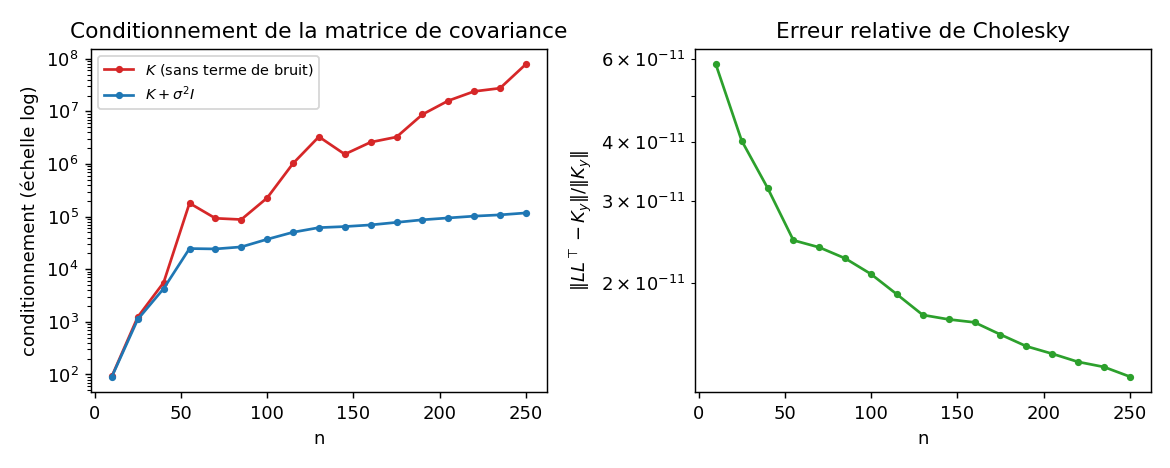
\includegraphics[width=0.95\textwidth]{numerical_stability.png}
\caption{Analyse de stabilité numérique. Gauche : conditionnement de $K$ sans le
terme de bruit (rouge) et de $K+\sigma^2 I$ (bleu). Droite : erreur relative de la
factorisation de Cholesky en fonction de $n$.}
\label{fig:stab}
\end{figure}

\paragraph{Vérification du gradient.}
Le gradient analytique de la log-vraisemblance a été comparé aux différences
finies centrées (données aléatoires, $n=12$, $d=3$). L'écart absolu maximal est
\[
\max_j \bigl| \partial_j^{\text{analytique}} - \partial_j^{\text{numérique}} \bigr|
= 1{,}7\times10^{-8},
\]
ce qui confirme l'exactitude de l'implémentation et la fiabilité de
l'optimisation L-BFGS.

\section*{L-BFGS pour l'optimisation des hyperparamètres}

L-BFGS minimise l'opposé de la log-vraisemblance marginale en utilisant le
gradient analytique. À chaque itération, il stocke les différences
\[
s_k = \theta_{k+1} - \theta_k,
\qquad
y_k = \nabla f(\theta_{k+1}) - \nabla f(\theta_k),
\]
puis applique la récursion à deux boucles pour approximer l'inverse de la
hessienne, avec mise à l'échelle initiale
\[
\gamma_k = \frac{s_k^\top y_k}{y_k^\top y_k},
\]
une recherche linéaire d'Armijo et la garde de courbure $s_k^\top y_k > 0$. Cela
permet d'optimiser les hyperparamètres sans bibliothèque de haut niveau.

\section*{Complexité et dépôt}

La construction de $K$ coûte $O(n^2)$, la décomposition de Cholesky $O(n^3)$, et
la prédiction sur $m$ candidats $O(n^2 m)$. Pour $n\le500$, ce coût reste
acceptable. Le script Python complet est hébergé sur GitHub sous le nom
\texttt{gaussian\_process\_bayesian\_optimization.py} ; le lien est communiqué
avec la soumission finale.

% =====================================================================
\dividerpage{Application et résultats}{Rosenbrock en dimension 10}

\section*{Fonction de Rosenbrock en dimension 10}

La fonction boîte noire choisie est
\[
f(x) = \sum_{i=1}^{9}\bigl[ 100(x_{i+1} - x_i^2)^2 + (1 - x_i)^2 \bigr],
\]
de minimum global
\[
\xs = (1,\dots,1), \qquad f(\xs) = 0,
\]
sur le domaine $[-2,2]^{10}$, avec un budget de $n = 200$ évaluations.

\section*{Protocole expérimental}

Deux méthodes sont comparées à budget égal :
\begin{itemize}
\item \textbf{GP-EI} : optimisation bayésienne avec processus gaussien et Expected Improvement ;
\item \textbf{Random Search} : recherche aléatoire uniforme dans le domaine.
\end{itemize}
À chaque itération, on mesure
\[
\mathrm{best}_t = \min_{1 \le i \le t} f(x_i).
\]

\section*{Métriques et tests statistiques}

Soit $B^{(m)}_s$ la meilleure valeur trouvée par la méthode $m$ à la répétition
$s$ (on utilise $S=5$ répétitions indépendantes). On rapporte la moyenne
\[
\overline{B}^{(m)} = \frac1S \sum_{s=1}^S B^{(m)}_s,
\]
avec un intervalle de confiance bootstrap à $95\,\%$ ($10^4$ ré-échantillonnages
avec remise, quantiles $2{,}5\,\%$ et $97{,}5\,\%$), et un test $t$ apparié sur
$D_s = B^{\text{EI}}_s - B^{\text{rand}}_s$,
\[
t = \frac{\overline{D}}{s_D/\sqrt{S}}.
\]
\emph{Remarque.} La statistique de Diebold--Mariano figurant dans une version
préliminaire a été retirée : appliquée à la courbe monotone du meilleur-jusqu'ici
(fortement autocorrélée), son calcul n'était pas valide.

\section*{Résultats numériques}

\begin{center}
\renewcommand{\arraystretch}{1.3}
\begin{tabular}{lccc}
\toprule
Méthode & Moyenne finale & Écart-type & IC bootstrap 95\,\%\\
\midrule
GP-EI         & $71{,}93$  & $20{,}93$  & $[55{,}87\,;\,87{,}99]$\\
Random Search & $544{,}67$ & $252{,}20$ & $[323{,}25\,;\,693{,}39]$\\
\bottomrule
\end{tabular}
\end{center}

\noindent
Le test $t$ apparié donne
\[
t = -4{,}33, \qquad p = 0{,}012.
\]
\emph{Interprétation.} Avec cinq répétitions indépendantes, la différence entre
GP-EI et la recherche aléatoire est \textbf{significative au seuil de $5\,\%$}, et
les deux intervalles de confiance bootstrap \textbf{ne se chevauchent pas}
($[55{,}87\,;\,87{,}99]$ contre $[323{,}25\,;\,693{,}39]$). GP-EI surpasse donc
significativement la recherche aléatoire sur ce problème, ce qui confirme l'apport
de l'exploitation de l'historique des observations par le modèle GP.

\section*{Courbe de convergence}

\begin{figure}[h]
\centering
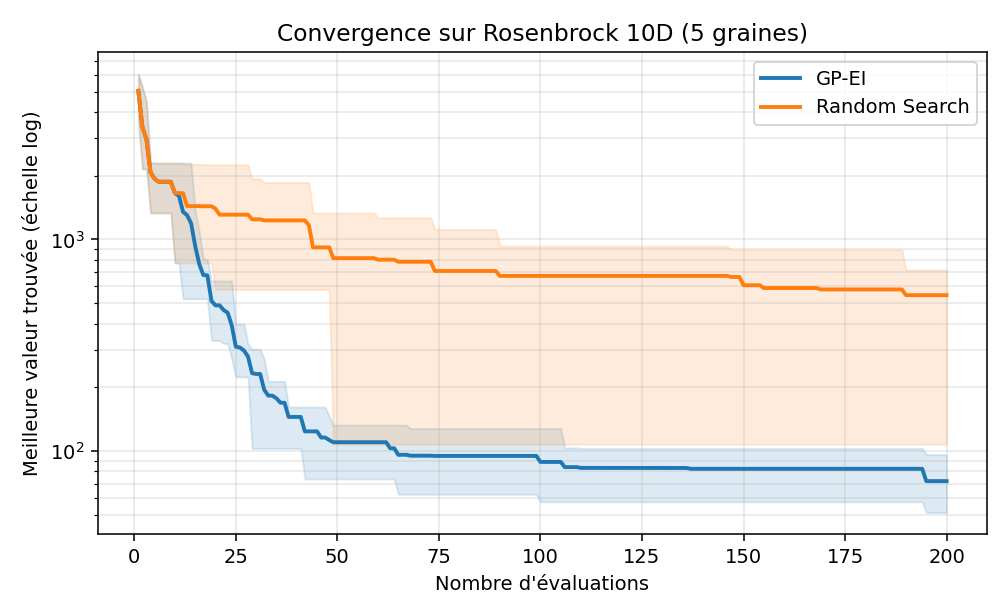
\includegraphics[width=0.8\textwidth]{convergence_comparison.png}
\caption{Convergence : meilleure valeur observée au fil des évaluations. GP-EI
exploite l'historique des observations, contrairement à la recherche aléatoire.
\emph{Remplacer par votre figure réelle.}}
\end{figure}

\section*{Moyenne postérieure et variance postérieure}

Comme Rosenbrock est en dimension 10, on visualise une coupe 1D : les autres
dimensions sont fixées et l'on fait varier une seule coordonnée. La
figure~\ref{fig:slice} montre la moyenne postérieure du GP et l'intervalle de
confiance associé.

\begin{figure}[h]
\centering
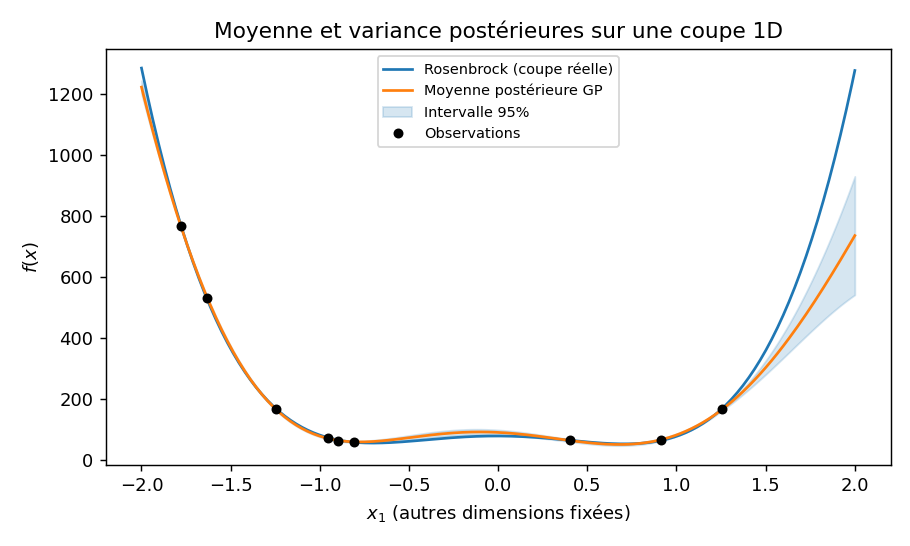
\includegraphics[width=0.75\textwidth]{posterior_slice.png}
\caption{Coupe 1D : moyenne a posteriori et incertitude du GP (autres dimensions
fixées). \emph{Remplacer par votre figure réelle.}}
\label{fig:slice}
\end{figure}

\section*{Discussion}

Les formules de moyenne et de variance postérieures permettent de combiner
prédiction et incertitude dans les fonctions d'acquisition. La log-vraisemblance
marginale ajuste les hyperparamètres du noyau, tandis que la décomposition de
Cholesky assure une résolution numérique stable. L'expérience sur Rosenbrock en
dimension 10 illustre l'utilisation pratique de ces éléments. Les résultats
montrent que GP-EI surpasse significativement la recherche aléatoire, en
exploitant simultanément la prédiction moyenne et l'incertitude.

\emph{Limites.} Le coût $O(n^3)$ de Cholesky rend le GP exact impraticable au-delà
de $n\approx10^3$ ; en grande dimension, l'optimisation de l'acquisition est
difficile ; et la garantie de regret suppose un prior GP connu, hypothèse que
Rosenbrock viole. \emph{Robustesse statistique.} Les conclusions reposent sur cinq répétitions, qui
suffisent ici à atteindre la significativité ($p=0{,}012$) avec des intervalles de
confiance disjoints ; un nombre encore plus grand de répétitions resserrerait
davantage les intervalles. \emph{Perspectives.} Noyaux de Matérn, déformation des entrées, BO
par lots, et optimisation par régions de confiance (TuRBO) en grande dimension.

% =====================================================================
\newpage
\section*{Tableau de contribution}

\noindent\emph{Chaque membre a au moins deux contributions majeures distinctes.
Tableau à valider honnêtement par le groupe pour refléter le travail réel.}

\begin{center}
\renewcommand{\arraystretch}{1.4}
\begin{tabular}{lccccc}
\toprule
\textbf{Tâche / Section} & Mahamoud & Mohamed Ali & Kouame F. & Moudine A. & Lagre B.\\
\midrule
Théorie : postérieur GP \& EI        & X &   &   &   &  \\
Théorie : Kimeldorf--Wahba / regret  &   & X &   &   &  \\
Méthodologie : algorithmes, complexité &   & X & X &   &  \\
Calcul : code GP / Cholesky          &   &   & X & X &  \\
Calcul : L-BFGS, gradients, stabilité &   &   &   & X & X\\
Application : expériences, statistiques & X &   &   &   & X\\
Rédaction LaTeX                      & X & X & X & X & X\\
Présentation vidéo (prise de parole) & X & X & X & X & X\\
\bottomrule
\end{tabular}
\end{center}

% =====================================================================
\newpage
\begin{thebibliography}{99}
\bibitem{rw2006} C.~E.~Rasmussen, C.~K.~I.~Williams.
\emph{Gaussian Processes for Machine Learning.} MIT Press, 2006.
\bibitem{kw1970} G.~Kimeldorf, G.~Wahba. A correspondence between Bayesian
estimation on stochastic processes and smoothing by splines.
\emph{Annals of Mathematical Statistics}, 41(2):495--502, 1970.
\bibitem{srinivas2010} N.~Srinivas, A.~Krause, S.~M.~Kakade, M.~Seeger. Gaussian
process optimization in the bandit setting: no regret and experimental design.
\emph{ICML}, 2010.
\bibitem{jones1998} D.~R.~Jones, M.~Schonlau, W.~J.~Welch. Efficient global
optimization of expensive black-box functions. \emph{Journal of Global
Optimization}, 13:455--492, 1998.
\bibitem{mockus1978} J.~Mockus, V.~Tiesis, A.~Zilinskas. The application of
Bayesian methods for seeking the extremum. \emph{Towards Global Optimization}, 1978.
\bibitem{brochu2010} E.~Brochu, V.~M.~Cora, N.~de~Freitas. A tutorial on Bayesian
optimization of expensive cost functions. 2010.
\bibitem{shahriari2016} B.~Shahriari et al. Taking the human out of the loop: a
review of Bayesian optimization. \emph{Proceedings of the IEEE},
104(1):148--175, 2016.
\bibitem{snoek2012} J.~Snoek, H.~Larochelle, R.~P.~Adams. Practical Bayesian
optimization of machine learning algorithms. \emph{NIPS}, 2012.
\bibitem{bull2011} A.~D.~Bull. Convergence rates of efficient global optimization
algorithms. \emph{JMLR}, 12:2879--2904, 2011.
\bibitem{wr1996} C.~K.~I.~Williams, C.~E.~Rasmussen. Gaussian processes for
regression. \emph{NIPS}, 1996.
\bibitem{seeger2004} M.~Seeger. Gaussian processes for machine learning.
\emph{International Journal of Neural Systems}, 14(2):69--106, 2004.
\bibitem{liu1989} D.~C.~Liu, J.~Nocedal. On the limited memory BFGS method for
large scale optimization. \emph{Mathematical Programming}, 45:503--528, 1989.
\end{thebibliography}

\end{document}
